\section{Design og Implementering}

\subsection{Kontrolinterfacet}
I dette afsnit beskrives design og implementering af Kontrolinterfacet som lavet på baggrund af kravspecifikationen og systemarkitekturen. 

Designet af Kontrolinterfacet afspejler meget den generelle opbygning af systemet. Således er hvert element af systemet implementeret som en klasse. Derudover er der nogle hjælpeklasser. En oversigt over klasserne og deres ansvar kan ses i tabel \ref{table:KI-klasser}.

Det gælder for VBTE-, SM- og Sensor-klasserne at når der efterspørges en af de værdier, klassen har ansvaret for, så benyttes RS232-objektet til at fremskaffe disse værdier ved hjælp af den serielle kommunikationsprotokol.


\begin{figure}[H]
\centering
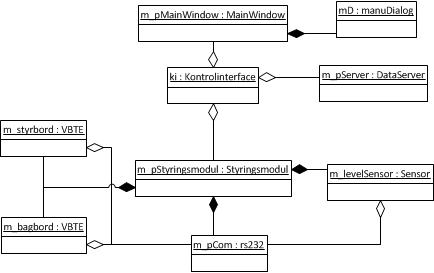
\includegraphics[width = 0.9\textwidth]{billeder/Objektdiagram}
\caption{Oversigt over, og sammenhæng mellem, objekter i kontrolinterface-programmet}
\label{fig:objektdiagram}
\end{figure}


\begin{table}[H]
\centering
\begin{tabular}{p{3cm} p{12.5cm}}
\multicolumn{2}{l}{{\Large Kontrolinterfacets klasser}} \\\hline
Kontrolinterface (KI)&Programmets hovedklasse. Eksisterer for at rydde op i main-funktionen.\\\\
DataServer (DS)&Står for alt TCP-kommunikationen med databasen. Oprettes af KI-klassen\\\\
Styringsmodul (SM)&Oprettes af KI og opretter VBTE-, Sensor- og RS232klasserne.\\\\
Sensor&Oprettes af SM og er ansvarlig for hældningsværdien. Når objektet bliver spurgt til den værdi af SM-klassen vil Sensor-klassen anvende sin delte association til RS232-objektet til at få denne af det fysiske SM-modul.\\\\
VBTE&Der eksisterer et VBTE-objekt for hvert fysisk VBTE-modul. Det er objektets ansvar at holde styr på værdierne for sit VBTE-modul.\\\\
RS232&Driveren til kommunikationen med det fysiske SM-modul. Objektet formidler sig på en protokol forstået af det tilsvarende objekt på SM-modulet. Objektet oprettes af SM-klassen og VBTE- og Sensorobjekterne har en delt association til den.\\\\
MainWindow&Oprettes af KI-klassen og kontrollerer og overvåger den grafiske brugergrænsefalde.\\\\
manudialog&Oprettes af MainWindow og styrer den dialog, der fremkommer når man ønsker en manuel hældningsregulering.\\\\
\end{tabular}
\caption{Kontrolinterfacets klasser}
\label{tabel:ki-klasser}
\end{table}